\documentclass[10pt]{beamer}
\usetheme[progressbar=frametitle]{metropolis}
\usecolortheme{moloch}
\useoutertheme{metropolis}
\useinnertheme{metropolis}
\usefonttheme{metropolis}
\usepackage[utf8]{inputenc}
\usepackage[T2A]{fontenc}
\usepackage[russian]{babel}
\usepackage{graphicx}
\usepackage{amsmath}
\usepackage{listings}
\usepackage{xcolor}
\usepackage{tabularx}

\title{Исследование и разработка методов автоматического профилирования автора русскоязычного текста}
\author{ИИПАмд-21 Филиппов Никита Андреевич}
\date{Научный руководитель: доцент кафедры ИС Воронина В.В. }

\begin{document}

\begin{frame}
\titlepage
\end{frame}

\section{Введение}

\begin{frame}{Предметная область}
\begin{block}{Высокие требования к цифровым сервисам}
Современные пользователи ожидают качественные и клиентоориентированные услуги. Бизнес стремится к повышению ключевых метрик: релевантным показам рекламы, высокой конверсии и снижению стоимости привлечения клиента
\end{block}

\begin{block}{Проблема недостатка данных}
Основная сложность в достижении этих показателей - отсутствие достоверной информации о пользователе сервиса. Традиционное ручное заполнение профилей (возраст, пол, интересы) часто игнорируется или сознательно искажается пользователями. По этой причине классические алгоритмы плохо справляются с задачей
\end{block}

\begin{block}{Решение через анализ текста}
Текст представляет собой цифровой отпечаток личности автора. Через его анализ можно извлечь множество характеристик, связанных с автором. Эта задача называется автоматическим профилированием текста
\end{block}
\end{frame}

\begin{frame}{Актуальность}
\begin{block}{Бизнес-применение автоматического профилирования}
Автоматическое профилирование автора текста позволяет решать ключевые бизнес-задачи цифровых платформ: персонализацию контента, таргетирование рекламы и глубокую аналитику аудитории без зависимости от ручного ввода данных.
\end{block}

\begin{itemize}
\item \textbf{Бизнес-потребность:} необходимость в персонализации, точном таргетинге и аналитике аудитории для улучшения ключевых метрик - снижения стоимости привлечения клиента, повышения показателя кликабельности и конверсии

\item \textbf{Недостаток традиционных подходов:} текущие алгоритмы оказываются неэффективными при неполной или недостоверной информации о пользователе

\item \textbf{Масштаб данных:} экспоненциальный рост пользовательского контента требует автоматизированных решений для анализа

\item \textbf{Отсутствие готовых решений:} недосаток решений для автоматического профилирования русскоязычных текстов
\end{itemize}
\end{frame}

\section{Цели и задачи}
\begin{frame}{Цель исследования}
Разработка и экспериментальное обоснование веб-сервиса для автоматического профилирования автора текста, направленного на повышение точности персонализации цифровых платформ.
\end{frame}

\begin{frame}{Задачи исследования}
\begin{enumerate}
\item Обзор методов и подходов к автоматическому профилированию
\item Выбор и адаптация методов для русского языка
\item Разработка процесса извлечения и подготовки признаков
\item Обучение моделей машинного обучения
\item Проектирование и реализация веб-сервиса
\item Экспериментальная оценка и анализ результатов
\end{enumerate}
\end{frame}

\begin{frame}{Объект и предмет}
\begin{itemize}
\item \textbf{Объект:} Процессы и методы анализа текстов для выявления характеристик автора
\item \textbf{Предмет:} Алгоритмы и программные решения для автоматического профилирования автора русскоязычного текста
\end{itemize}
\end{frame}

\begin{frame}{Научная новизна исследования}
\begin{block}{Контекст исследования}
Работа представляет собой системное исследование и практическую реализацию методов автоматического профилирования автора текста, адаптированных для русскоязычных текстов.
\end{block}

\begin{itemize}
\item \textbf{Адаптация и систематизация существующих методов:} Проведено комплексное исследование современных подходов к автоматическому профилированию с учётом специфики русского языка

\item \textbf{Формализация процесса профилирования:} Разработана формальная модель системы автоматического профилирования, обеспечивающая воспроизводимость результатов

\item \textbf{Практическая реализация системы:} Создан работающий программный комплекс, объединяющий различные методы профилирования в единой системе с веб-интерфейсом и API
\end{itemize}
\end{frame}

\section{Методология}

\begin{frame}{Состав профиля автора текста}
\begin{block}{Ключевые атрибуты профиля}
Авторский профиль может включать различные характеристики: демографические, социальные, психологические и поведенческие. Среди них выделяются \textbf{первичные атрибуты} — пол и возраст, которые оказывают наиболее значимое влияние на стиль письма и служат основой для определения остальных характеристик.
\end{block}

\begin{block}{Выбор атрибутов для исследования}
В рамках данной работы для анализа выбраны \textbf{пол} и \textbf{возрастная группа} автора. Этот выбор обусловлен следующими причинами:
\begin{itemize}
\item Наличие размеченных данных для русского языка (корпус BlogsGenderAge)
\item Хорошо изученные лингвистические маркеры
\item Прямое практическое применение в задачах персонализации
\end{itemize}
\end{block}
\end{frame}

\begin{frame}{Модель 'Как есть'}

\begin{figure}

\includegraphics[width=0.8\textwidth]{images/as-is-full.png}
% \caption{Модель 'Как есть'}
\end{figure}

\begin{itemize}
\item Зависимость от профильных данных
\item Низкая релевантность таргетинга
\item Высокий CAC
\end{itemize}

\end{frame}

\begin{frame}{Модель 'Как должно быть'}

\begin{figure}

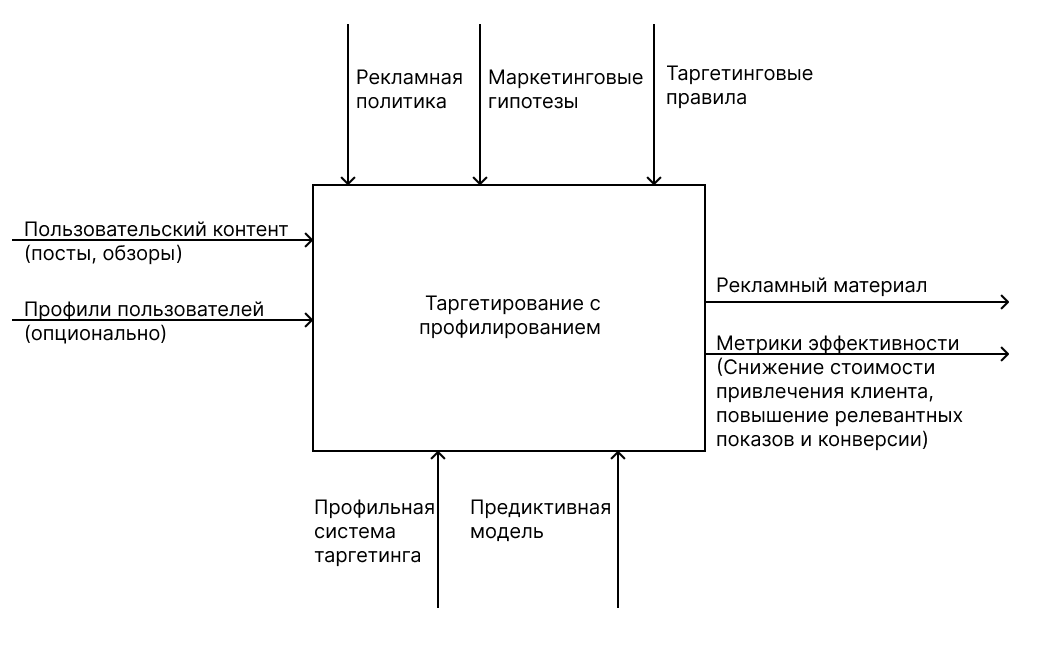
\includegraphics[width=0.8\textwidth]{images/to-be.png}
% \caption{Модель 'Как должно быть'}
\end{figure}

\begin{itemize}
\item Интеграция модуля автоматического профилирования
\item Обогащение профилей на основе контента
\item Повышение релевантности и снижение CAC
\end{itemize}

\end{frame}

\begin{frame}{Cуществующие решения}
\footnotesize
\begin{table}[]
\centering
\resizebox{\textwidth}{!}{%
\begin{tabular}{|p{1.8cm}|p{5cm}|p{4.2cm}|}
\hline
\textbf{Система} & \textbf{Основная функция} & \textbf{Ограничения для задачи профилирования} \\
\hline
Bukvik LitTerra &  Платформа для анализа текста: POS-разметка, анализ тональности, сетевой анализ, этимологический анализ, относительная энтропия  & Фокус на атрибуции авторства и сравнительном анализе текстов \\
\hline
RuLex & Оценка сложности и читабельности текстов & Специализирован на оценке читабельности и педагогических метриках \\
\hline
Textometr & Многофункциональный лингвистический анализатор (сложность, читаемость, лексическое разнообразие, ключевые слова) & Cпециализирован на оценке читабельности и педагогических метриках \\
\hline
\end{tabular}
}
\end{table}

\normalsize

\begin{block}{Вывод}
\begin{itemize}
\item Существующие решения предоставляют отдельные компоненты, которые могут быть использованы для извлечения признаков
\item Ни одна из рассмотренных систем не решает задачу автоматического составления демографического профиля автора
\end{itemize}
\end{block}
\end{frame}

\begin{frame}{Подходы извлечения информации из текста}

\textbf{Стилометрический подход:} лексика, морфология, синтаксис, пунктуация, TTR, длины слов/предложений
\begin{itemize}
\item Фокус на формальных характеристиках
\item Устойчивость к тематическим сдвигам
\item Меньшая зависимость от домена
\item Чувствителен к объёму текста, уязвим к обфускации
\end{itemize}

\textbf{Контекстный подход:} ключевые слова, тематика, NER
\begin{itemize}
\item Фокус на тематике и семантике
\item Высокая интерпретируемость
\item Сильная зависимость от домена
\end{itemize}
\end{frame}

\begin{frame}{Подходы в классификации составного профиля}
\begin{columns}[T]
\begin{column}{0.48\textwidth}
\textbf{Плоская классификация}
\begin{itemize}
\item Одна модель для всех атрибутов
\item Простота реализации
\item Экспоненциальный рост классов
\item Не работает в случае гетерогенных целевых переменных
\end{itemize}
\end{column}
\begin{column}{0.48\textwidth}
\textbf{Иерархическая классификация}
\begin{itemize}
\item Последовательное уточнение атрибутов
\item Использование специализированных моделей
\item Более высокая точность
\end{itemize}
\end{column}
\end{columns}
\end{frame}

\section{Теоретическое описание системы}

\begin{frame}{Алгоритм обработки документа}
\begin{figure}

\includegraphics[width=\textwidth, height=0.8\textheight, keepaspectratio]{images/doc-processing.png}
\caption{Алгоритм обработки документа}
\end{figure}
\end{frame}

\begin{frame}{План обучения моделей}
\begin{itemize}
\item \textbf{Модели:} LR, SVM, Naive Bayes, KNN, RF, GBM, MLP
\item \textbf{Гиперпараметры:} Подбор через GridSearchCV
\item \textbf{Критерии:} Accuracy, Precision, Recall, F1-score, Матрицы ошибок
\item \textbf{Валидация:} 5-фолдовая кросс-валидация
\end{itemize}
\end{frame}

\section{Проектирование системы}

\begin{frame}{Диаграмма вариантов использования}
\begin{figure}
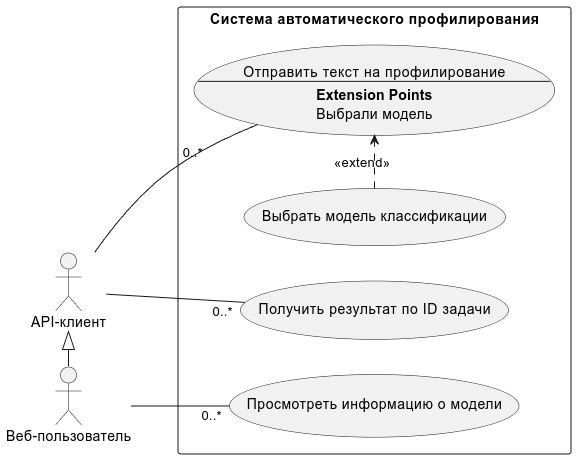
\includegraphics[width=0.8\textwidth]{images/use-case.png}
\caption{Варианты использования системы}
\end{figure}
\end{frame}

\begin{frame}{Диаграмма классов системы}
\begin{figure}
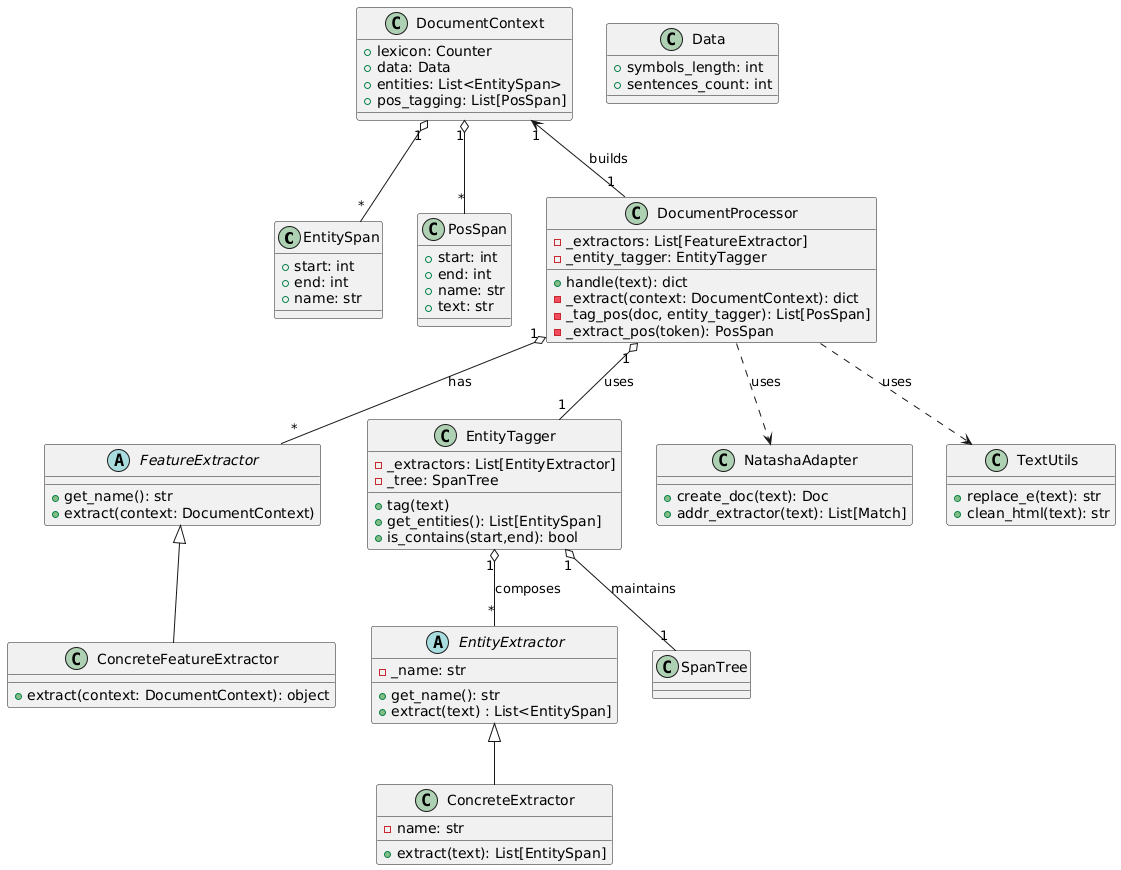
\includegraphics[width=0.8\textwidth]{images/nlp.png}
\caption{Архитектура классов системы}
\end{figure}
\end{frame}

\begin{frame}{Диаграмма последовательности}
\begin{figure}

\includegraphics[width=0.8\textwidth]{images/seq.png}
\caption{Последовательность обработки запроса}
\end{figure}
\end{frame}

\begin{frame}{Диаграмма компонентов}
\begin{figure}
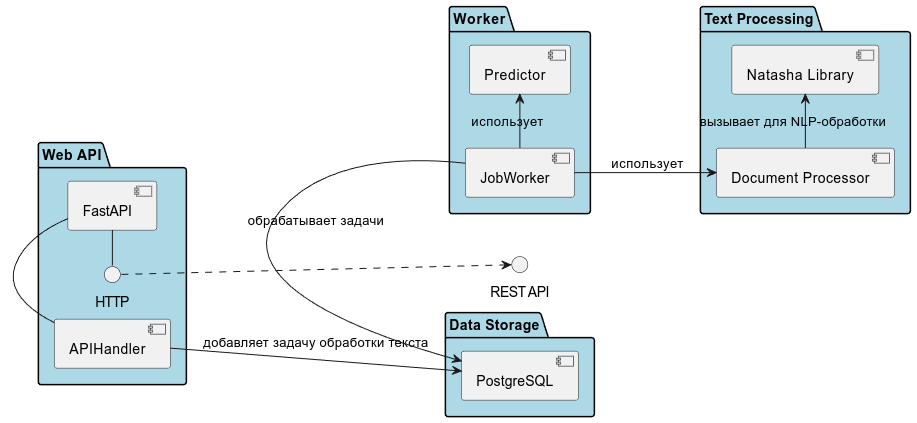
\includegraphics[width=0.8\textwidth]{images/comp.png}
\caption{Компонентная архитектура системы}
\end{figure}
\end{frame}

\begin{frame}{Архитектура развертывания системы}
\begin{figure}
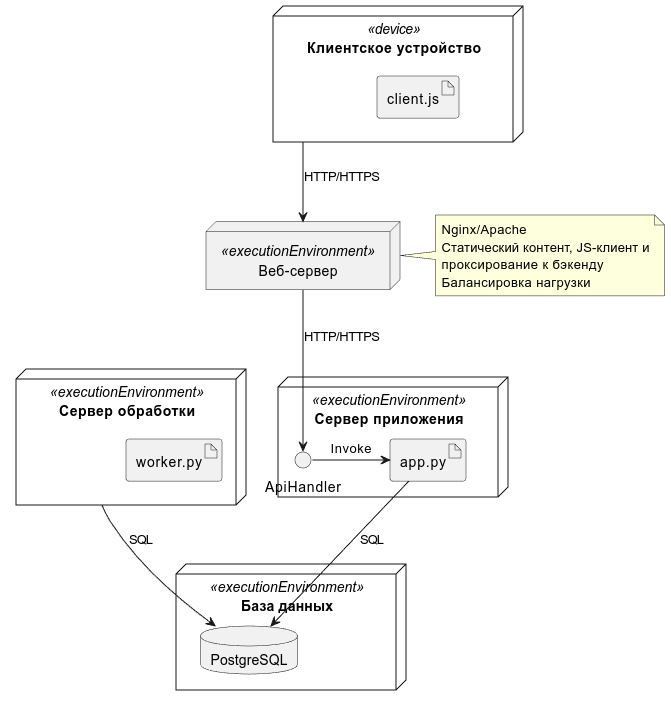
\includegraphics[width=\textwidth, height=0.8\textheight, keepaspectratio]{images/depl.png}
\caption{Архитектура развертывания}
\end{figure}
\end{frame}

\begin{frame}{Интерфейс пользователя. Главная страницаа}
\begin{figure}

\includegraphics[width=\textwidth]{images/main-page.png}
\end{figure}
\end{frame}

\begin{frame}{Интерфейс пользователя. Результат профилирования}
\begin{figure}

\includegraphics[width=\textwidth]{images/profile-page.png}
\end{figure}
\end{frame}

\begin{frame}{Интерфейс пользователя. Информация о модели}
\begin{figure}
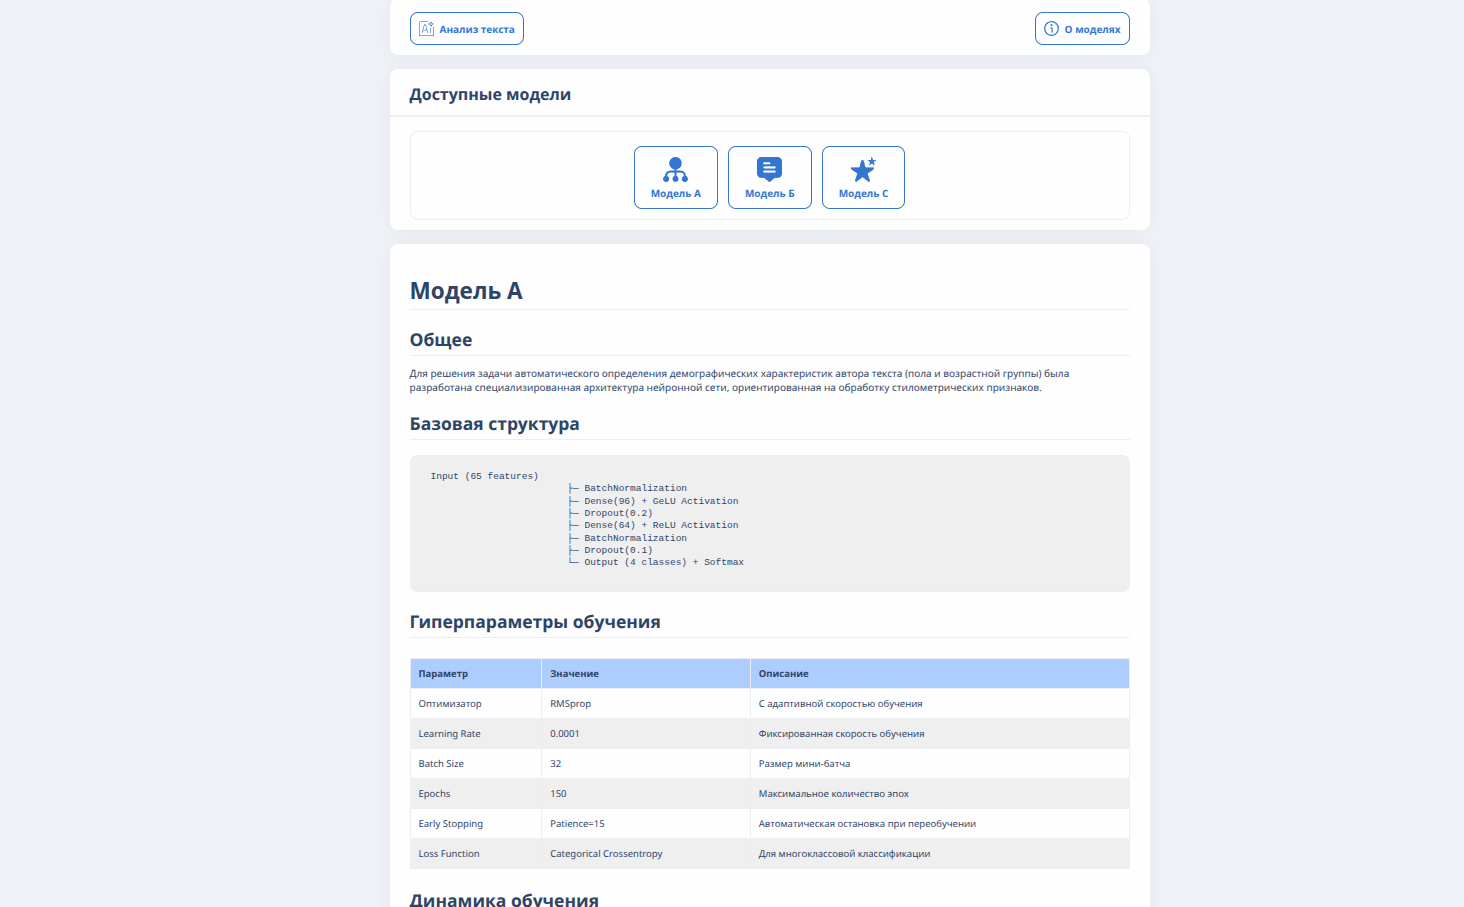
\includegraphics[width=\textwidth]{images/model-info-page.png}
\end{figure}
\end{frame}


\begin{frame}{Используемые технологии}
\begin{itemize}
\item Python: FastAPI, Scikit-learn, Pandas, Numpy, Seaborn, Matplotlib, Scipy, Keras
\item NLP: Natasha, pymorphy2, nltk
\item База данных: PostgreSQL
\item Веб-сервер: Nginx
\item Клиент: jQuery, Panini, Gulp
\item Асинхронная обработка: Celery
\end{itemize}
\end{frame}

\section{Текущее состояние проекта}
\begin{frame}{Текущее состояние}
\begin{block}{Текущий статус}
Разработан черновой прототип системы автоматического профилирования, включающий:
\begin{itemize}
\item Базовый пайплайн обработки текстовых данных
\item Набор моделей машинного обучения для определения пола и возраста
\item Веб-интерфейс для взаимодействия с системой
\end{itemize}
\end{block}
\end{frame}

\begin{frame}{Задачи на доработку}
    
\begin{block}{Задачи на доработку}
\begin{enumerate}
\item \textbf{Повторная предобработка данных} с учётом корректировок и требований от предприятия
\item \textbf{Разведывательный анализ данных} для выявления новых закономерностей и улучшения признакового пространства
\item \textbf{Обучение и эксперименты} с моделями с учётом обновлённых задач и требований
\item \textbf{Доведение прототипа до рабочего состояния} — интеграция, тестирование, оптимизация
\item \textbf{Подготовка примеров использования} и оформление информационных материалов
\end{enumerate}
\end{block}

\end{frame}

\begin{frame}
\centering
\Large Спасибо за внимание!\\
\vspace{1cm}
\large Вопросы?
\end{frame}


\end{document}
